\documentclass[journal]{IEEEtran}

\usepackage{newtxtext,newtxmath}
\usepackage{graphicx}
\usepackage{booktabs}
\usepackage{amsmath}
\usepackage{url}
\usepackage[hidelinks]{hyperref}
\graphicspath{{../results/}}

\begin{document}

\title{Transfer Learning in CNNs: Comparing Training from Scratch, Feature Extraction, and Fine-Tuning on a Small Flower Dataset}

\author{Ron~John~Galvez,
        Venz~Gerolaga,
        Brian~David~Metrillo,
        and~John~Mark~Romero
\thanks{The authors are with the Department of Electronics, Computer, and Electrical Engineering, Gokongwei College of Engineering, De La Salle University, Manila, Philippines.}
\thanks{Code and results: \url{https://github.com/Shujimaki/cpecog2-transfer-minilab}}}

\markboth{CPECOG2 Deep Neural Networks, Transfer Learning Mini-Lab}{Galvez \MakeLowercase{\textit{et al.}}: Transfer Learning in CNNs}

\maketitle

\begin{abstract}
Training a convolutional neural network (CNN) from scratch needs far more labeled images than most small projects have. Transfer learning reuses a network pretrained on a large dataset instead. This paper compares four strategies on a 5-class flower dataset with 300 images per class: a small CNN trained from scratch, and an ImageNet-pretrained ResNet-50 used for feature extraction, partial fine-tuning, and full fine-tuning. Each model was trained on 10\%, 25\%, 50\%, and 100\% of a 900-image training set and tested on a fixed 300-image test set. All three transfer strategies beat the scratch CNN by 22 to 30 percentage points at every training-set size. Partial fine-tuning, which retrains only the last residual stage and the classifier, gave the best accuracy at 25\% and 50\% of the data (88.0\% and 91.0\%). At 10\% and 100\%, the three transfer strategies were within 2 points of each other. Full fine-tuning reached the highest accuracy overall, 93.0\%, but needed about twice the training time per epoch. The results agree with the guideline that a small target dataset similar to the source should keep most of the pretrained backbone fixed.
\end{abstract}

\begin{IEEEkeywords}
Transfer learning, convolutional neural networks, ResNet-50, fine-tuning, feature extraction, image classification.
\end{IEEEkeywords}

\section{Introduction}
\IEEEPARstart{M}{odern} CNNs have millions of parameters. ResNet-50 has 25.6 million, while a typical course or lab project has only hundreds to a few thousand labeled images. A randomly initialized network of that size overfits a small dataset. Transfer learning addresses this by reusing what a model learned on a large source task, such as ImageNet classification, for a smaller target task~\cite{pan2010survey}.

Transfer works because CNN features are hierarchical. Early layers detect edges and color blobs that are useful for nearly any image, while later layers become specific to the source classes~\cite{zeiler2014visualizing,yosinski2014transferable}. In practice, this gives a spectrum of strategies. Feature extraction keeps the pretrained backbone frozen and trains only a new classifier. Fine-tuning also retrains some or all of the backbone at a small learning rate.

This paper carries out the CPECOG2 transfer learning mini-lab. It answers one question: on a small, natural-image dataset, which strategy gives the best accuracy at each training-set size, and at what cost? We report accuracy, macro-F1, the number of trainable parameters, and training time for four models, and we plot accuracy against training-set size.

\section{Related Work}
Yosinski \textit{et al.}~\cite{yosinski2014transferable} measured how transferable each layer of an AlexNet-style network is. They found that early layers transfer almost without loss, that the transfer gap grows toward higher layers, and that fine-tuned transferred layers generalize better than training from scratch. Razavian \textit{et al.}~\cite{razavian2014cnn} showed that a linear classifier on frozen ImageNet features is a strong baseline for many recognition tasks. Pretraining does not always win, however. He \textit{et al.}~\cite{he2019rethinking} matched pretrained results on COCO detection by training from scratch for long enough. Kornblith \textit{et al.}~\cite{kornblith2019better} found that pretraining helped little on some fine-grained datasets. Raghu \textit{et al.}~\cite{raghu2019transfusion} found limited gains for some medical imaging tasks. These studies suggest that the benefit of transfer depends on how much target data is available and how close the target is to the source, which is what this experiment tests.

\section{Methodology}

\subsection{Dataset}
We used the TF Flowers dataset~\cite{tfflowers}, which has 3,670 photographs in five classes: daisy, dandelion, roses, sunflowers, and tulips. The classes contain 633 to 898 images each. The mini-lab asks for 200 to 500 images per class, so we randomly kept 300 images per class with a fixed seed, for 1,500 images in total. We split them once, stratified by class, into 900 training, 300 validation, and 300 test images (60/20/20). Every model and every training-set size used this same split.

For the size sweep, we drew stratified subsets of 10\%, 25\%, 50\%, and 100\% of the training set, which is 90, 225, 450, and 900 images. The subsets are nested, so the 10\% subset is part of the 25\% subset, and so on. The validation and test sets never changed.

All images were resized to $224\times224$ pixels and normalized with the ImageNet channel mean and standard deviation, which the pretrained weights expect. The training set used random horizontal flips as its only augmentation.

\subsection{Models}
\textit{Scratch CNN:} three convolutional blocks (Conv $3\times3$, BatchNorm, ReLU, $2\times2$ max pooling) with 32, 64, and 128 filters, followed by global average pooling, dropout of 0.3, and a linear layer with five outputs. It has 94,341 parameters, all randomly initialized.

\textit{ResNet-50 strategies:} all three start from the torchvision ResNet-50 with ImageNet weights~\cite{he2016deep,deng2009imagenet} (\texttt{IMAGENET1K\_V2}). We replaced the original $2048\times1000$ classifier with a new $2048\times5$ layer, which has 10,245 parameters.
\begin{itemize}
\item \textit{Feature extraction:} the whole backbone is frozen, and only the new classifier trains.
\item \textit{Partial fine-tuning:} the classifier and the last residual stage (\texttt{layer4}) train. This is 14,974,981 parameters.
\item \textit{Full fine-tuning:} all 23,518,277 parameters train.
\end{itemize}

\subsection{Training}
All models used the Adam optimizer~\cite{kingma2015adam}, cross-entropy loss, and a batch size of 32. The scratch CNN used a learning rate of $10^{-3}$. For the transfer models, the new classifier used $10^{-3}$ and the backbone used $10^{-4}$, which is ten times smaller so that the pretrained weights change slowly.

Partial and full fine-tuning began with a two-epoch warm-up in which only the classifier trained. A random classifier produces large gradients that can damage the pretrained weights, so the backbone was unfrozen only after the warm-up. In all ResNet-50 models, the BatchNorm layers~\cite{ioffe2015batch} kept their pretrained running statistics during training. Updating them with small batches of new data makes them noisy.

Training used early stopping on validation loss with a patience of three epochs, and the weights with the lowest validation loss were restored. The epoch limits were 30 for the scratch CNN, 40 for feature extraction, and 10 for partial and full fine-tuning. Feature extraction needs more epochs because each epoch makes only a few updates to a small classifier. Training time was measured as wall-clock time on an Apple M2 GPU (MPS) using PyTorch~\cite{paszke2019pytorch}. Every run used the same random seed.

\subsection{Evaluation}
Each trained model was evaluated once on the fixed test set. We report accuracy and macro-F1, which is the unweighted mean of the per-class F1 scores. With 300 test images, one image is 0.33 percentage points. Because we used a single seed, we treat differences of 2 points (6 images) or less as ties.

\section{Results}

\subsection{Full Training Set}
Table~\ref{tab:full} shows the four models trained on all 900 training images. The three transfer strategies reached 91.0\% to 93.0\% accuracy, while the scratch CNN reached 69.0\%. Macro-F1 closely matched accuracy for every model because the classes are balanced. Full fine-tuning was the most accurate and partial fine-tuning was second, but the gap between them is 2 test images. Feature extraction trained the fewest parameters yet took the longest total time. Each of its epochs still runs the full ResNet-50 forward pass, and it needed 35 epochs before early stopping. Per epoch, the times were 8.9~s for the scratch CNN, 14.4~s for feature extraction, 18.6~s for partial fine-tuning, and 33.8~s for full fine-tuning.

\begin{table}[!t]
\caption{Results on the Full Training Set (900 Images)}
\label{tab:full}
\centering
\begin{tabular}{@{}lrrrr@{}}
\toprule
Model & Acc. & Macro-F1 & Trainable & Time (s) \\
\midrule
Scratch CNN        & 0.690 & 0.689 & 94,341     & 106 \\
Feature extraction & 0.910 & 0.910 & 10,245     & 503 \\
Partial FT         & 0.923 & 0.924 & 14,974,981 & 112 \\
Full FT            & 0.930 & 0.930 & 23,518,277 & 270 \\
\bottomrule
\end{tabular}
\end{table}

\subsection{Accuracy Against Training-Set Size}
Fig.~\ref{fig:size} and Table~\ref{tab:size} show test accuracy for each training-set size. The scratch CNN improved from 54.3\% to 69.0\% as the training set grew, but it stayed 24 to 30 points below the best model at every size. Partial fine-tuning was the most accurate at 25\% and 50\%, ahead of the other two transfer strategies by 2.3 points (7 test images) both times. At 10\%, the three transfer strategies were within 2 points of each other. At 100\%, full fine-tuning was highest, but again within 2 points of the others.

At 10\% and 25\%, feature extraction used all 40 epochs while its validation loss was still falling, by 0.002 to 0.004 per epoch. Those two accuracies are therefore slight underestimates.

\begin{figure}[!t]
\centering
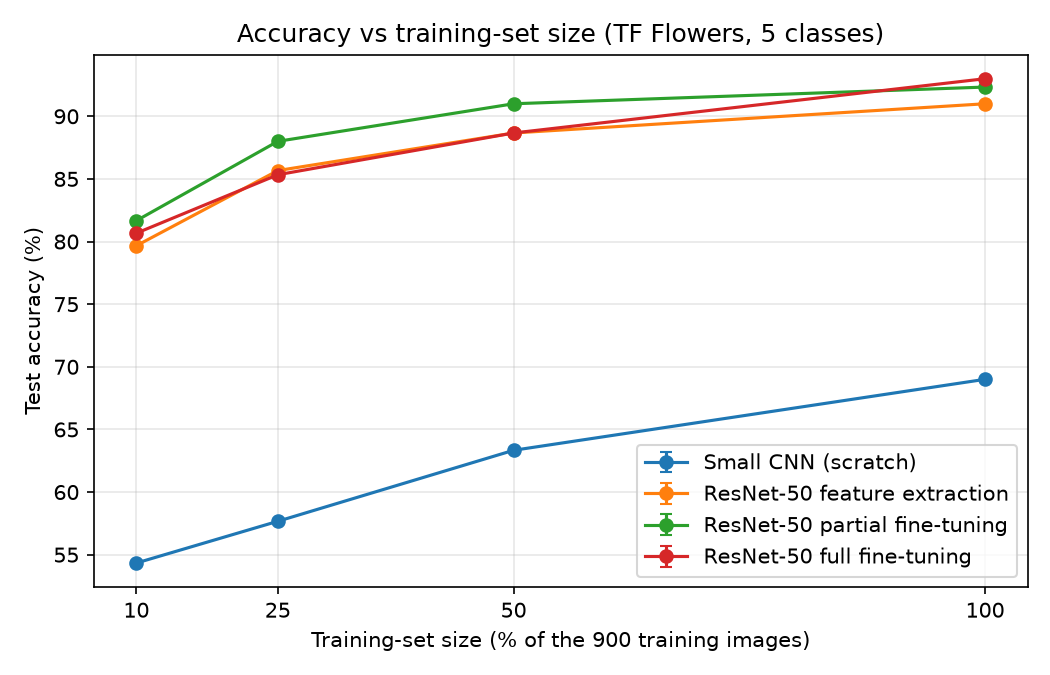
\includegraphics[width=\columnwidth]{accuracy_vs_size.png}
\caption{Test accuracy against training-set size for the four strategies. The x-axis is the percentage of the 900 training images used.}
\label{fig:size}
\end{figure}

\begin{table}[!t]
\caption{Test Accuracy by Training-Set Size}
\label{tab:size}
\centering
\begin{tabular}{@{}lrrrr@{}}
\toprule
Train images & Scratch & Feat. ext. & Partial FT & Full FT \\
\midrule
90 (10\%)   & 0.543 & 0.797 & \textbf{0.817} & 0.807 \\
225 (25\%)  & 0.577 & 0.857 & \textbf{0.880} & 0.853 \\
450 (50\%)  & 0.633 & 0.887 & \textbf{0.910} & 0.887 \\
900 (100\%) & 0.690 & 0.910 & 0.923 & \textbf{0.930} \\
\bottomrule
\end{tabular}
\end{table}

\subsection{Per-Class Errors}
Fig.~\ref{fig:cm} shows the confusion matrix of the best model, full fine-tuning on the full training set. Dandelion was the easiest class (58 of 60 correct) and tulips the hardest (53 of 60). Tulips were most often mistaken for daisies and roses (3 each), and sunflowers for dandelions (4). These pairs share colors or petal shapes, so the remaining errors are between visually similar flowers.

\begin{figure}[!t]
\centering
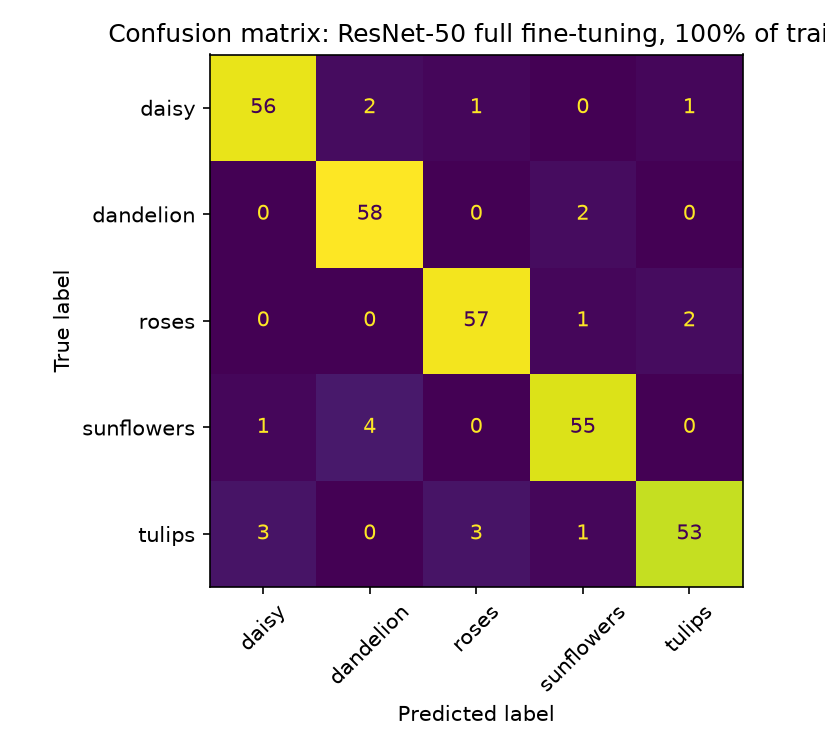
\includegraphics[width=0.85\columnwidth, trim=0 0 0 45, clip]{confusion_best.png}
\caption{Confusion matrix of full fine-tuning trained on 100\% of the training set (300 test images, 60 per class).}
\label{fig:cm}
\end{figure}

\section{Discussion}
Transfer learning was the largest effect in this experiment. Even the frozen backbone, which trains only 10,245 parameters, beat the scratch CNN by 22 to 28 points at every size. ResNet-50 already learned edges, textures, and object parts from 1.28 million ImageNet images, and flower photographs are close to ImageNet photographs, so these features carry over. The scratch CNN has to learn the same features from at most 180 images per class, and it was still improving when the data ran out.

Among the transfer strategies, partial fine-tuning gave the best balance. Feature extraction cannot change its features, which were learned for the 1,000 ImageNet classes, so it trailed partial fine-tuning at every size. Retraining \texttt{layer4}, the most task-specific stage, lets the network adapt to the small differences between flower species. The smaller backbone learning rate and the frozen BatchNorm statistics kept this adaptation from erasing the pretrained features. Full fine-tuning has 23.5 million parameters to fit, which gave no gain over partial fine-tuning with 450 images or fewer, and it cost about twice the time per epoch. With the full training set it caught up and reached the highest accuracy, although by a margin within our noise level.

This pattern matches the common guideline for choosing a strategy by data size and similarity to the source. For a small target dataset that is similar to the source, keep most of the backbone fixed and adapt only the top layers. As the dataset grows, unfreezing more layers starts to pay off. We did not test a target far from ImageNet, such as spectrograms or X-rays, where the guideline recommends fine-tuning more layers and where pretraining may help less~\cite{raghu2019transfusion}.

The main limitation of this study is that it uses one seed and a 300-image test set. Differences of a few images between the transfer strategies at 10\% and 100\% could change with another seed, so repeating each run over several seeds and reporting the mean and standard deviation would confirm those close cases. Feature extraction was also slightly undertrained at the two smallest sizes, so its true gap to partial fine-tuning there may be smaller than measured.

\section{Conclusion}
We compared a scratch CNN with three ResNet-50 transfer strategies on a 5-class flower dataset at four training-set sizes. Transfer learning improved accuracy by 22 to 30 points over training from scratch at every size. Partial fine-tuning was the best or tied for best at every size and was the clear winner at 25\% and 50\% of the data, at a training cost close to the scratch CNN. Full fine-tuning reached the highest accuracy, 93.0\%, only with the full training set and at about twice the cost per epoch. For a small dataset of natural images, fine-tuning only the top of a pretrained network is the most practical choice.

\begin{thebibliography}{99}

\bibitem{pan2010survey}
S.~J. Pan and Q.~Yang, ``A survey on transfer learning,'' \textit{IEEE Trans. Knowl. Data Eng.}, vol.~22, no.~10, pp.~1345--1359, Oct. 2010.

\bibitem{zeiler2014visualizing}
M.~D. Zeiler and R.~Fergus, ``Visualizing and understanding convolutional networks,'' in \textit{Proc. Eur. Conf. Comput. Vis. (ECCV)}, 2014.

\bibitem{yosinski2014transferable}
J.~Yosinski, J.~Clune, Y.~Bengio, and H.~Lipson, ``How transferable are features in deep neural networks?'' in \textit{Proc. Adv. Neural Inf. Process. Syst. (NeurIPS)}, 2014.

\bibitem{razavian2014cnn}
A.~S. Razavian, H.~Azizpour, J.~Sullivan, and S.~Carlsson, ``CNN features off-the-shelf: An astounding baseline for recognition,'' in \textit{Proc. IEEE Conf. Comput. Vis. Pattern Recognit. Workshops (CVPRW)}, 2014.

\bibitem{he2019rethinking}
K.~He, R.~Girshick, and P.~Doll\'{a}r, ``Rethinking ImageNet pre-training,'' in \textit{Proc. IEEE Int. Conf. Comput. Vis. (ICCV)}, 2019.

\bibitem{kornblith2019better}
S.~Kornblith, J.~Shlens, and Q.~V. Le, ``Do better ImageNet models transfer better?'' in \textit{Proc. IEEE Conf. Comput. Vis. Pattern Recognit. (CVPR)}, 2019.

\bibitem{raghu2019transfusion}
M.~Raghu, C.~Zhang, J.~Kleinberg, and S.~Bengio, ``Transfusion: Understanding transfer learning for medical imaging,'' in \textit{Proc. Adv. Neural Inf. Process. Syst. (NeurIPS)}, 2019.

\bibitem{tfflowers}
The TensorFlow Team, ``Flowers,'' 2019. [Online]. Available: \url{https://storage.googleapis.com/download.tensorflow.org/example_images/flower_photos.tgz}

\bibitem{he2016deep}
K.~He, X.~Zhang, S.~Ren, and J.~Sun, ``Deep residual learning for image recognition,'' in \textit{Proc. IEEE Conf. Comput. Vis. Pattern Recognit. (CVPR)}, 2016.

\bibitem{deng2009imagenet}
J.~Deng, W.~Dong, R.~Socher, L.-J. Li, K.~Li, and L.~Fei-Fei, ``ImageNet: A large-scale hierarchical image database,'' in \textit{Proc. IEEE Conf. Comput. Vis. Pattern Recognit. (CVPR)}, 2009.

\bibitem{kingma2015adam}
D.~P. Kingma and J.~Ba, ``Adam: A method for stochastic optimization,'' in \textit{Proc. Int. Conf. Learn. Represent. (ICLR)}, 2015.

\bibitem{ioffe2015batch}
S.~Ioffe and C.~Szegedy, ``Batch normalization: Accelerating deep network training by reducing internal covariate shift,'' in \textit{Proc. Int. Conf. Mach. Learn. (ICML)}, 2015.

\bibitem{paszke2019pytorch}
A.~Paszke \textit{et al.}, ``PyTorch: An imperative style, high-performance deep learning library,'' in \textit{Proc. Adv. Neural Inf. Process. Syst. (NeurIPS)}, 2019.

\end{thebibliography}

\end{document}
